% ........................................................................... %

This chapter introduces web services and the novelties brought by service-oriented computing for facilitating enterprise integration beyond the traditional boundaries of organizations information systems. Indeed, web services are not ``just'' an evolution of existing middleware, they also address new integration needs.

The structure of this chapter is the following. We start by a brief introduction to enterprise integration and application architectures. We then present some families of conventional middlewares that have been used for application integration, and we show their limitations in light of new integration challenges, including the need to facilitate integration between business partners.  We then present service-oriented computing and the business protocol model and analysis techniques that serve as a foundation of this thesis contributions.

% ........................................................................... %

\section{Enterprise integration}

% ........................................................................... %

The information system of an organization typically comprises various assets that range from data sources (e.g., relational databases systems) to applications that fulfill different needs (e.g., office tasks suites or business intelligence solutions). Such parts of an information system are either developed ``in-house'' to meet specific requirements, or they are acquired from third-party vendors (with possible customer-specific adaptations). Those assets rarely live isolated to each other. Indeed, it is often necessary for an application to access the data produced by another one, or even to access some parts of an API\footnote{Application Programming Interface.} to reuse some of its functionalities. Enterprise integration is a strong information technology concern \cite{HW03}. Careful practice is required to foster existing applications and stir their full potential in the larger view of an enterprise information system \cite{EAA02}.\\

Web services, and more generally service-oriented architectures, provide new perspectives for facilitating enterprise integration. They not only break technical barriers (e.g., difficulties in bridging applications from different organizations), they also enhance the architecture of information systems in a distributed, platform and language agnostic manner (e.g., bridging applications written in Cobol, Java and .Net). However, web services should not be viewed as \emph{revolutionary}. They should rather be seen as \emph{evolutionary}, i.e., they are an evolution of enterprise integration practices over the last few decades \cite{Alonso04}.\\

This section reviews the architectures found in enterprise applications, and highlight where integration can happen as it next focuses on middlewares\footnote{Briefly, the term \emph{middleware} designates software that facilitates the interoperability between heterogeneous systems.}.

% ........................................................................... %

\subsection{Application architectures}

% ........................................................................... %

\begin{figure}[htbp]
    \centering
    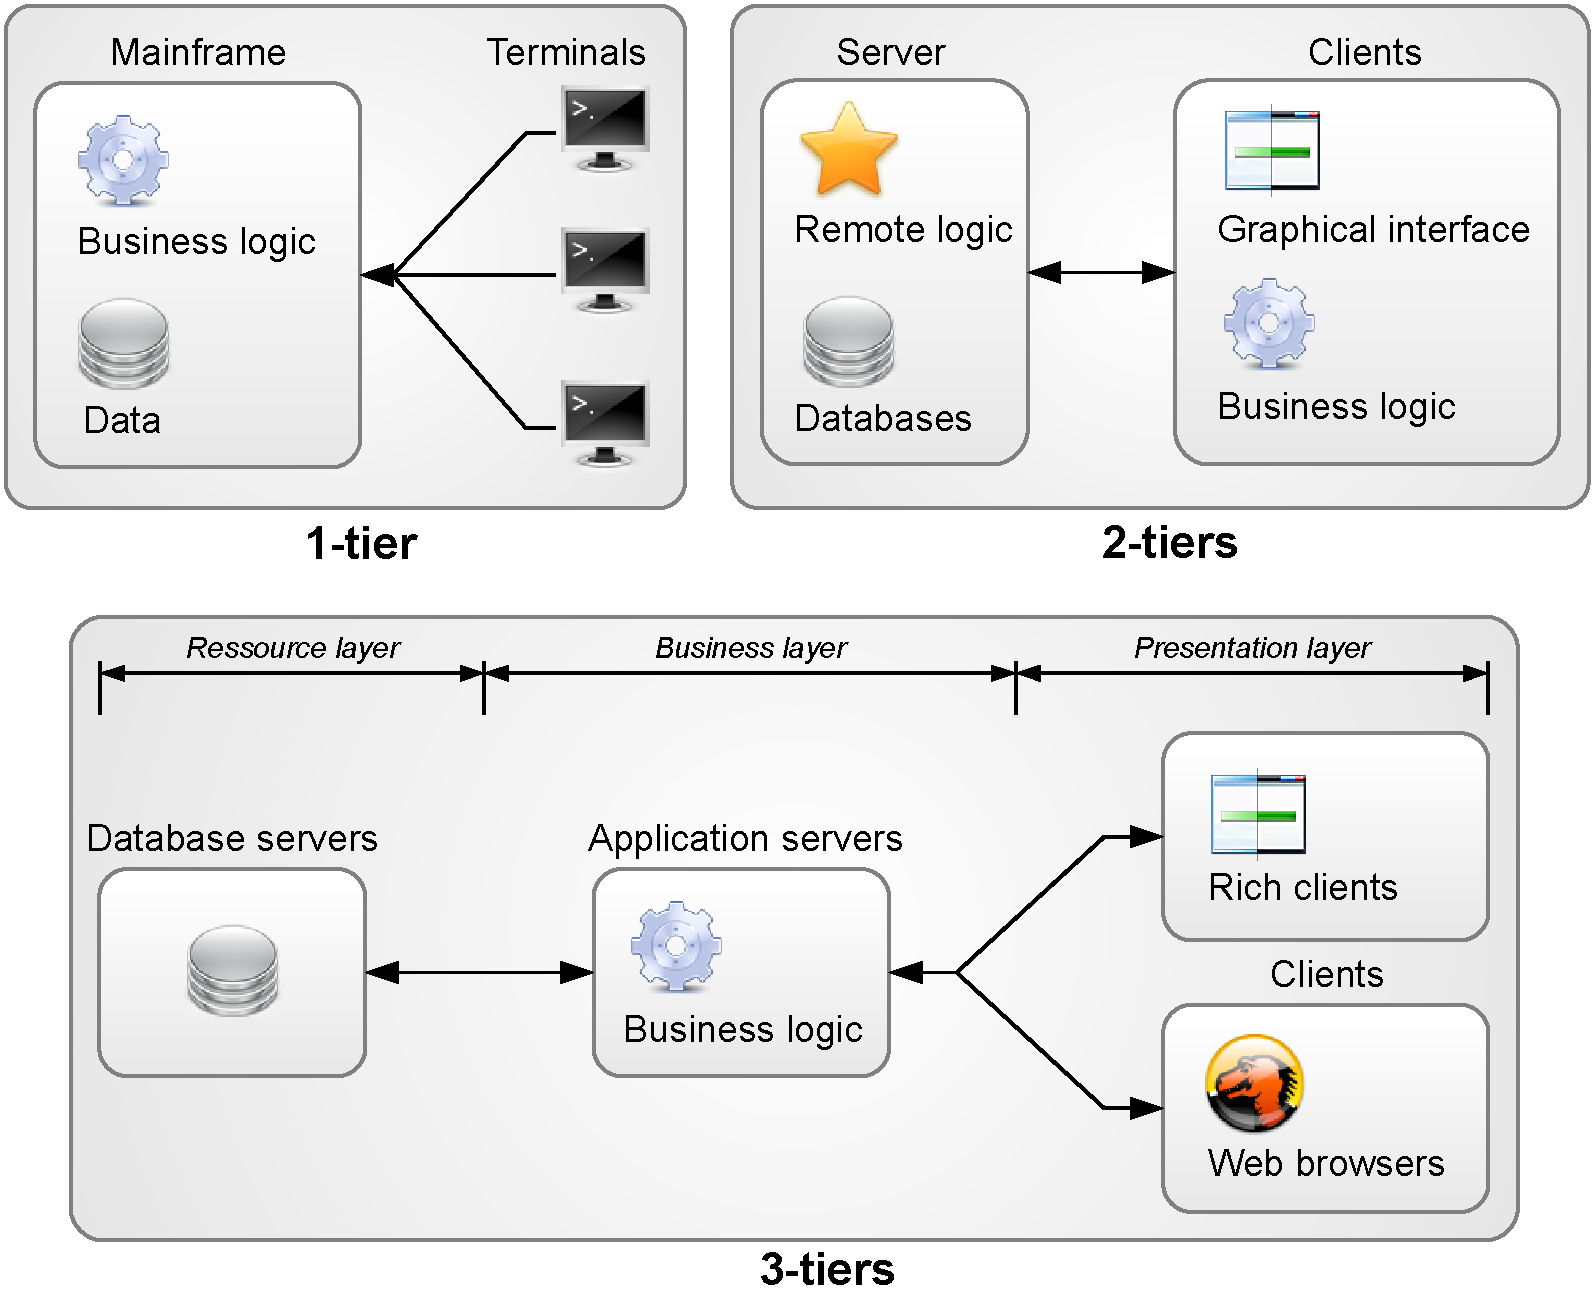
\includegraphics[width=\textwidth]{content/web-services/123-tiers}
    \caption{Overview of typical 1-tier, 2-tiers and 3-tiers architectures.}
    \label{fig:123-tiers}
\end{figure}

From an architectural point-of-view, it is common to differentiate different \emph{tiers} in an application. This is especially true with the generalization of distributed applications as the different tiers can be physically deployed separately \cite{Alonso04}. We briefly present the typical tiered architectures while an overview of them is available in Figure~\ref{fig:123-tiers}.

\paragraph{1-tier (70's -- 80's).}
This type of architecture is highly reminiscent of the early design of enterprise applications of the 70's and has kept being used throughout many developments of the 80's. Those architectures were relying on applications to be deployed on a single physical machine, called a \emph{mainframe}, while end-users would access it through \emph{terminals} over a network (often a proprietary network solution rather than a standards-based one). This type of architecture turned out to be relatively simple to run with simplified maintenance life-cycles as applications were deployed to a single, central machine. It had however a lot of obvious problems, including the need for expensive hardware upgrades to scale up in the number of concurrent terminals or the single-point of failure syndrome.

\paragraph{2-tiers (90's).}
This is also called \emph{client / server} in reference to the decomposition of the application units in server-side and client-side units. Those architectures have been primarily pushed forward by the generalization of relational database management systems exposed through network interfaces, thus providing an application neutral way for applications to store and gather data. The database systems are deployed server-side while the remainder of the application (business logic and visual interface) is client-side. There are variants to this: some computation-intensive tasks can be deported to the server as well. Also, some applications can embed client-side databases. A typical example of this is the support of ``offline modes'' where an application needs to store data when no network connection is available and synchronize it with the server when it becomes available again. Compared to 1-tier architectures, 2-tier applications brought a number of improvements, among which the promotion of standard-based networks as well as normalized data storage and representation systems. Performance-wise, they were also able to introduce clustering of both databases and portions of business logic to handle scalability in the number of clients.

\paragraph{3-tiers and $n$-tiers (end 90's -- 2000's).}
A 3-tiers application comprises the following layers \cite{HW03}.
\begin{itemize}
  
  \item The \emph{resources layer} provides an access to databases, files, network interfaces and legacy applications.
  
  \item The \emph{business layer} provides the core functionalities of applications, no matter how they are accessed. This layer often relies on component technologies (e.g., EJBs\footnote{Enterprise Java Beans}, see \url{http://java.sun.com/products/ejb/}).
  
  \item The \emph{presentation layer} exposes the applications to end-users and applications through a rich set of devices and technologies. In a similar fashion as the model--view--controller paradigm, the very same application can be exposed through different presentation interfaces.
  
\end{itemize}
This type of architecture started to become widespread with the advent of database-driven web applications. It pushed the generalization of \emph{application servers} (e.g., JavaEE, .Net Framework or LAMP\footnote{Acronym for Linux, Apache, MySQL and PHP / Perl / Python (this is not strict as other technologies can be used as replacements).} solutions) that embed the business logic, with the database storage being often delegated to another server. In turn, the presentation layer is accessed through web browsers which are light and generic display devices. Those applications can still be accessed from desktop applications, now called \emph{rich clients} by contrast to web browsers being considered as \emph{thin clients}. The term ``$n$-tiers'' refers to a finer-grained decomposition of an application architecture than 3-tiers. For example in the business layer, a purchase order management component may rely on a remote payment processing component.

\paragraph{Integration placeholders.}
Enterprise integration can be performed:
\begin{itemize}

	\item \emph{horizontally}, by integrating assets from the same tier (e.g., integrating data from heterogeneous customer-centric databases), and
	
	\item \emph{vertically}, by allowing the components from one tier to access to an upper or lower tier (e.g., a payroll management component accessing a relational database).

\end{itemize}
Integrating such assets would be easy in a perfect world where data representation and application interfaces would be uniform. The reality is of course very different as an information system present some of the following sources of heterogeneity: platforms (including operating systems, hardware architectures and execution platforms), databases systems and programming languages.

As an organization evolves, it periodically changes its technological standards, resulting in the need to  integrate new and legacy systems. For example a warehouse management application may have been developed a few years back using the \emph{Delphi} programming platform while new systems need to be developed in Java. Such legacy systems are often kept ``as-is'' since rewriting them has significant costs (e.g., development and training of employees) without necessarily resulting in practical benefits (e.g., the ``old'' application already fulfills the needs). \\

Systems that facilitate both horizontal and vertical enterprise applications integration are called \emph{middlewares}. The next section provides an overview of them.

% ........................................................................... %

\subsection{Middlewares}

% ........................................................................... %

In this section, we review some common middleware families. We also expose the limitations of conventional middlewares. The role of a middleware goes beyond just bridging heterogeneous software artifacts: it hides some of their inherent complexity (much like a \emph{Facade} does in object-oriented programming \cite{Gamma95}). A middleware can provide some development-time infrastructure (e.g., developer tools) and runtime infrastructure (e.g., deployed execution and monitoring components). We give a few examples of middlewares families \cite{Alonso04,HW03}. The platforms that are based on middleware technologies rarely support only a single family. Full-stack application servers such as the ones that provides the JavaEE specification implement much of the following ones.

\begin{figure}[htbp]
    \centering
    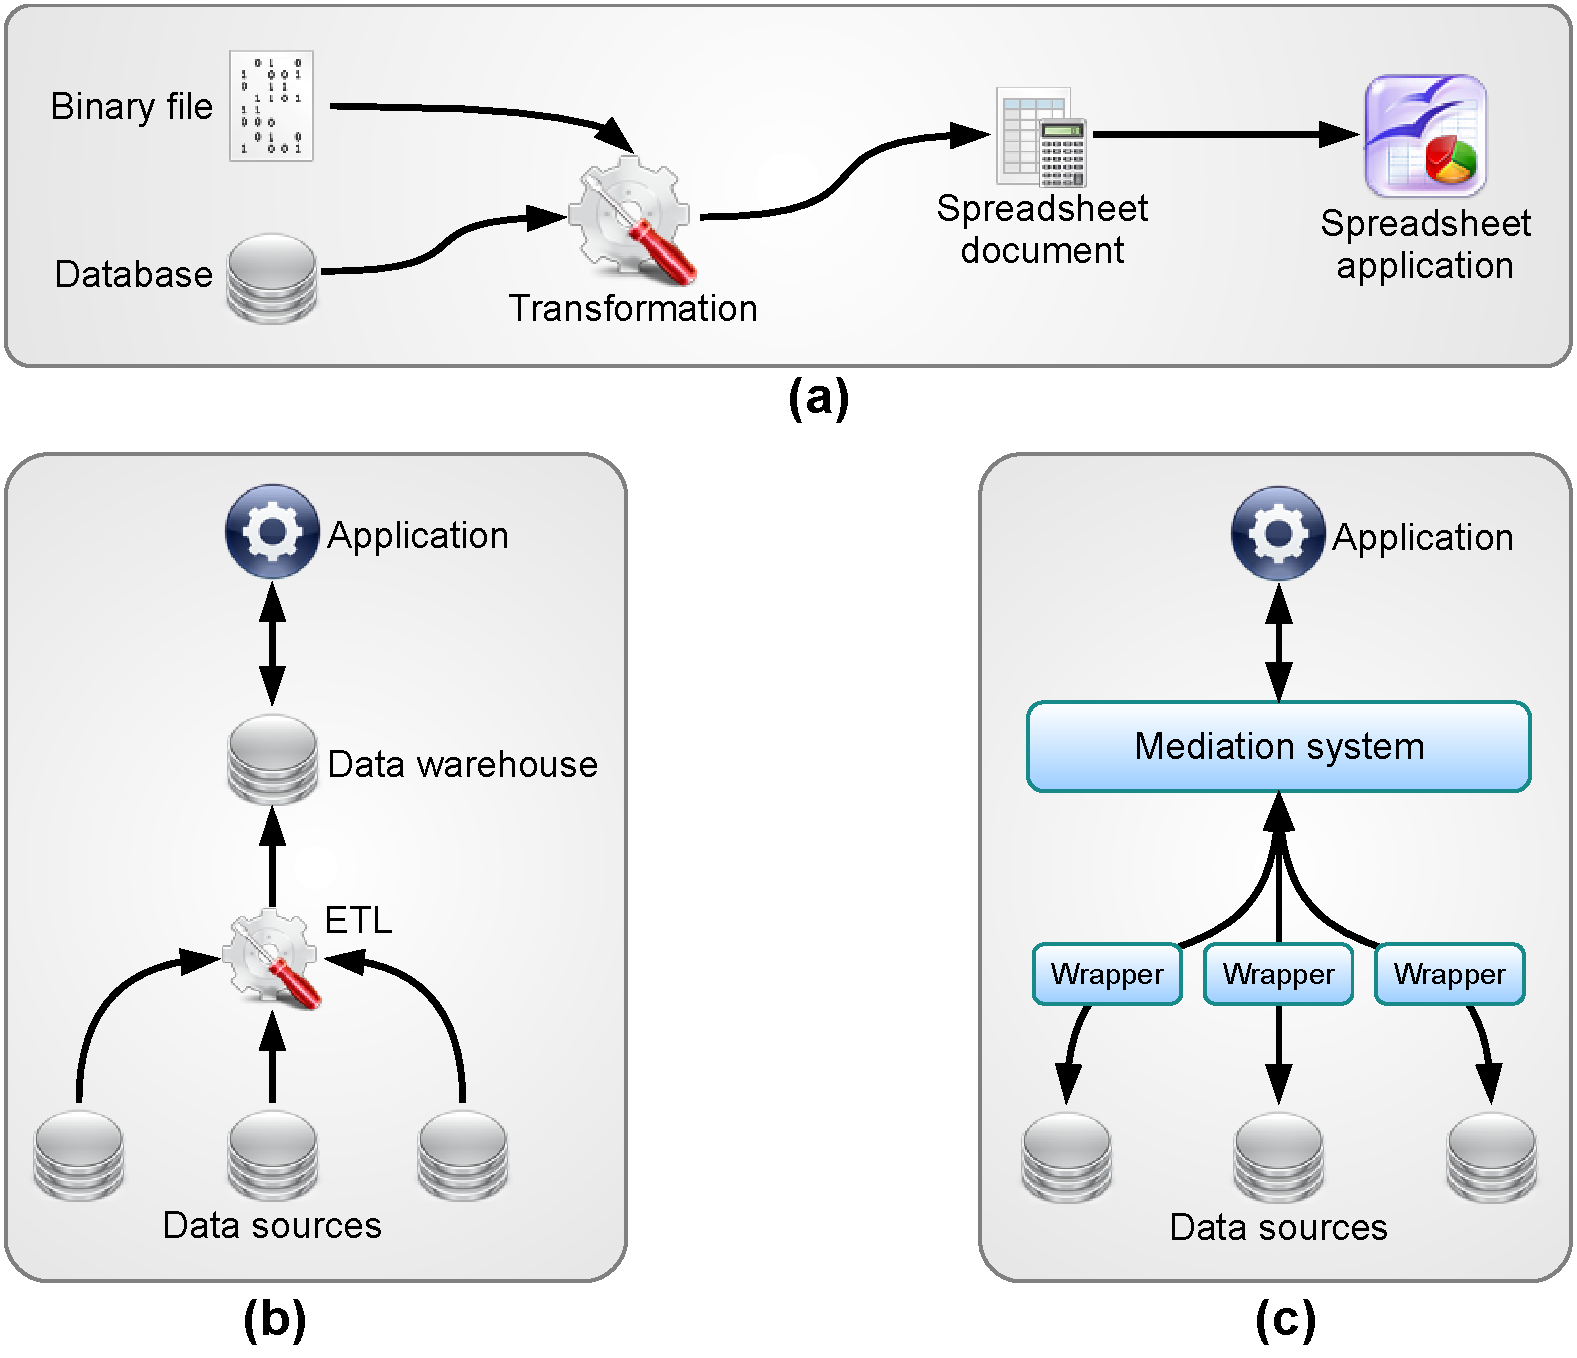
\includegraphics[width=\textwidth]{content/web-services/data-integration}
    \caption{Different approaches for data integration.}
    \label{fig:data-integration}
\end{figure}

\paragraph{Data integration.}
Applications physically store their data in files, databases, relational databases and so on. Several approaches exist, and we illustrated them on Figure~\ref{fig:data-integration}. The first one is to adapt the data from one or more applications so that another one can process it (Figure~\ref{fig:data-integration}(a)). An example would be to extract some data from a spreadsheet document and a relational database and transfer to another application. This involves creating ad-hoc transformation components (e.g., scripts or XSLT transformers). The other approach to data integration is to integrate data sources as heterogeneous, distributed relational databases. In this case there are two ways of achieving it.
\begin{enumerate}

	\item Materialized approaches use ETL\footnote{Extract, Transform and Load} tools that pull data from several relational database sources, normalize/transform it, then finally push it to \emph{data-warehouses} (Figure~\ref{fig:data-integration}(b)).
	
	\item Virtual approaches (Figure~\ref{fig:data-integration}(c)) use techniques and concepts such as \emph{global-as-view} and \emph{local-as-view} where the data is exposed by the mean of queries over the sources (see \cite{Ullman00,Lenzerini02} for an overview and \cite{ChawatheGHPUW94,LevyRO96,LattesR00,HalevyIMMST04} for implementation-related discussions).

\end{enumerate}

\begin{figure}[htbp]
    \centering
    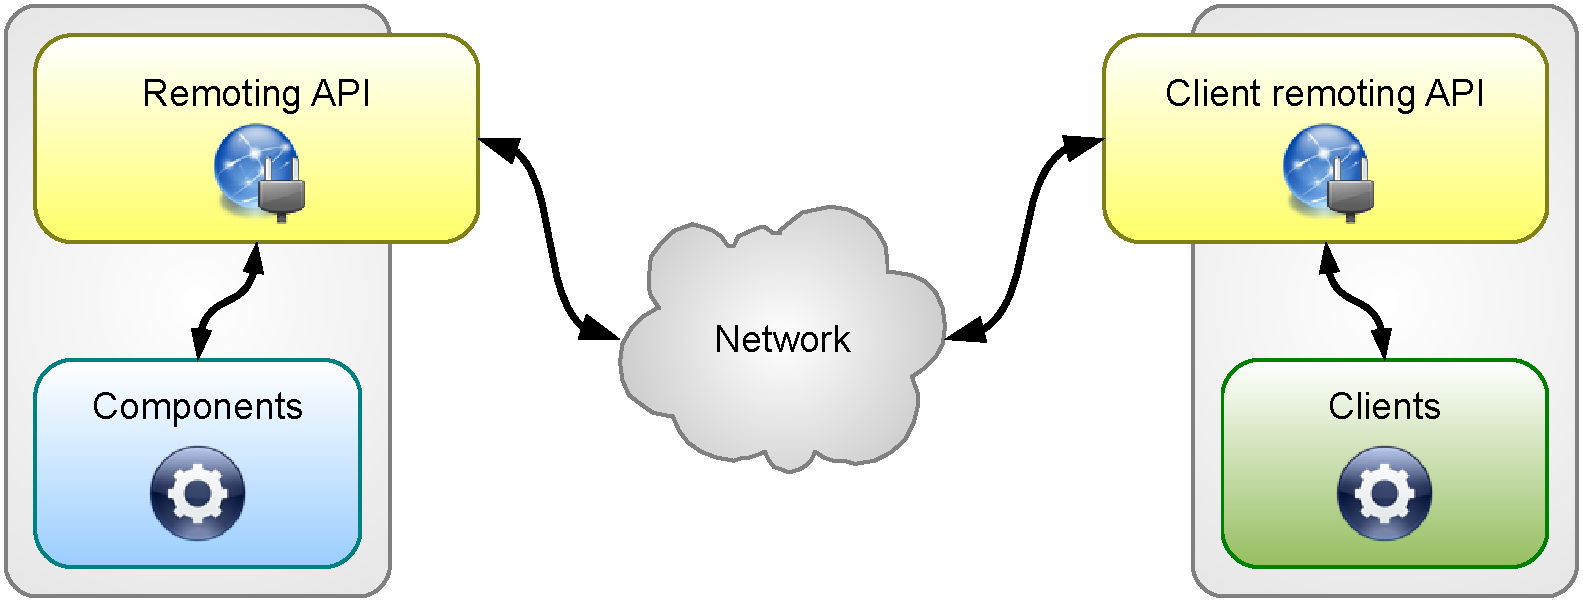
\includegraphics[width=\textwidth]{content/web-services/rpc-middleware}
    \caption{RPC-style middleware.}
    \label{fig:rpc-middleware}
\end{figure}

\paragraph{Remote procedure calls (RPC).}
They allow applications to communicate through regular \emph{procedure / function / method} calls of programming languages. Such a call looks like a normal, local invocation of some application code, but in reality, the actual code that is executed runs on a remote system. To do that, RPC middlewares encode the call parameters in a message that is sent over the network to the remote machine that will run the actual code. Once it has been executed, a response message is sent back to the invoking application with a return value being encoded inside the message. An illustration is provided on Figure~\ref{fig:rpc-middleware}. The preparation of the message (either for performing the call or returning the value) is called \emph{marshaling}. Similarly, the decoding of the message (either on the remote server or the invoker side) is called \emph{unmarshaling}. RCP middlewares have been implemented for a lot of languages and platforms. Examples include distributed components such as EJBs (remote session beans) or Microsoft DCOM.
  
\begin{figure}[htbp]
    \centering
    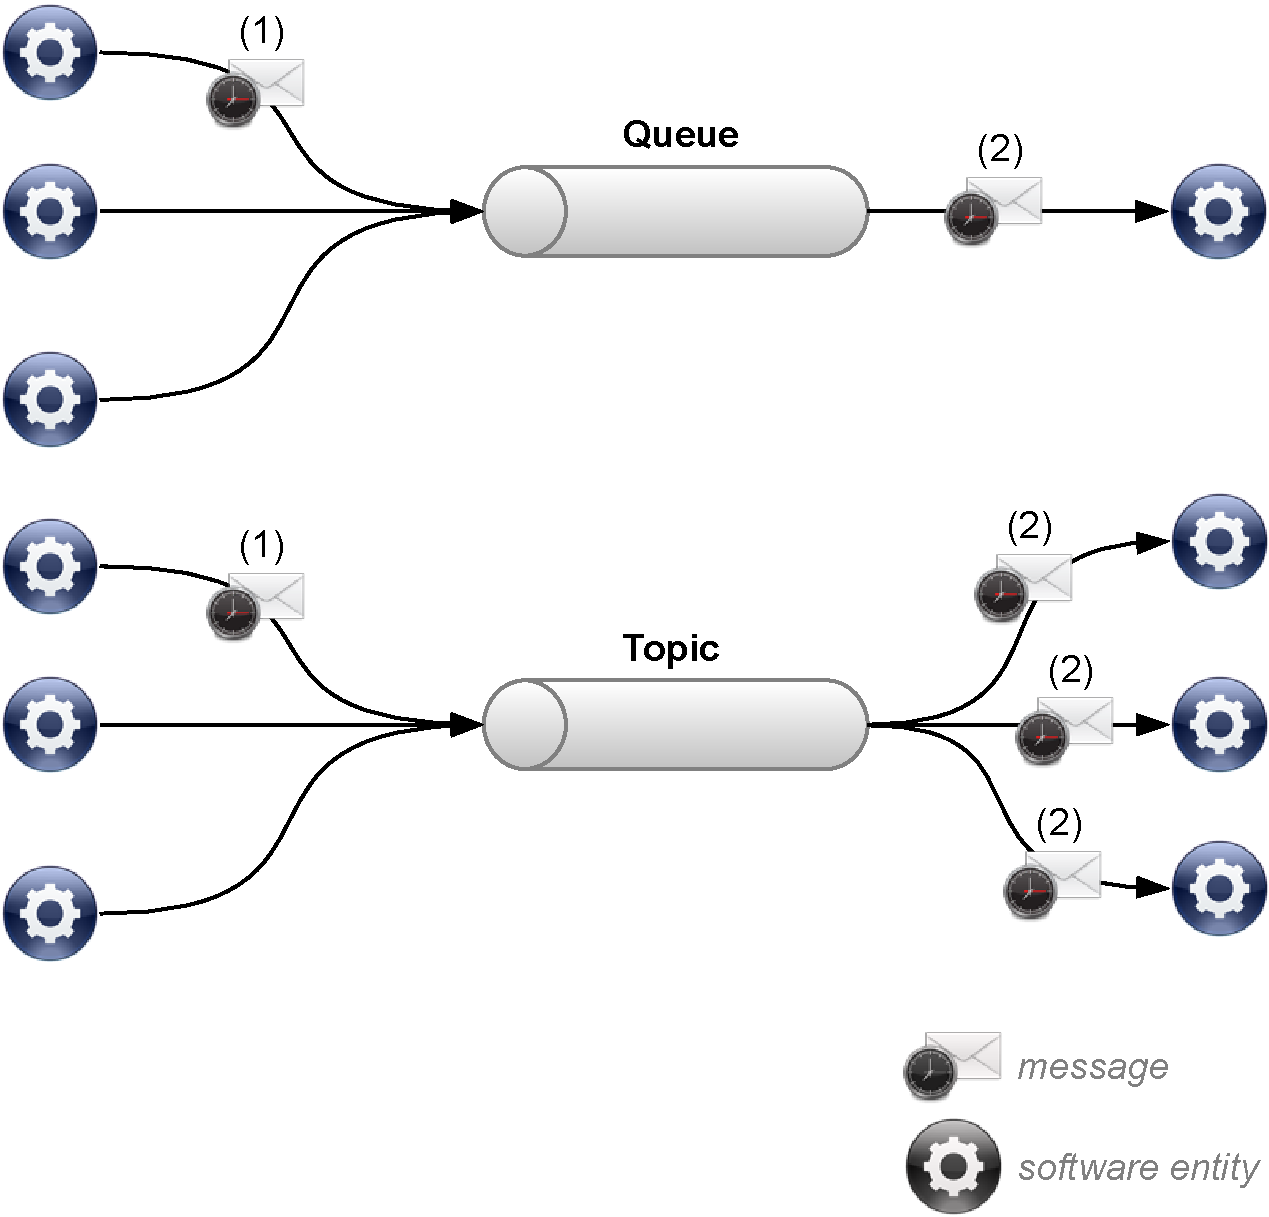
\includegraphics[width=0.8\textwidth]{content/web-services/messaging-middleware}
    \caption{Messaging middleware.}
    \label{fig:messaging-middleware}
\end{figure}
  
\paragraph{Message-oriented middlewares (MOM).}
They allow the communication between applications through asynchronous messages. By contrast to RPC middlewares, the messages do not cary ``function call'' semantics as they are rather general purpose documents exchanged between the systems. A MOM is responsible for collecting and routing messages. It also ensures their integrity, and that the messages are not being lost. Quality of service requirements are generally available, with priorities and validity expiration dates being the two most common in use. A MOM is also able to transform the message contents. This is useful when a message needs to be routed to an application that does not understand the initial message data format.
Two message basic communication patterns are found in MOM (see Figure~\ref{fig:messaging-middleware}): \emph{message queues} provide $n$-to-$1$ communication between $n$ message emitters and one receiver while \emph{message topics} allow broadcasting messages between $n$ emitters and $m$ receivers. An example specification of a MOM is the Java Messaging System (JMS).
  
\paragraph{Object request brokers (ORB).}
They allow clients to delegate the discovery and binding processes of components that match programmatic interfaces. The broker will select the best component according to the criteria it has been configured for, and will provide the clients with objects without them knowing what their concrete implementations are. To do that, an ORB relies on directories of components. Corba (\url{http://www.corba.org/}) is an example of a middleware comprising ORB technology.

\paragraph{Transaction monitors (TP).}
They ensure the coordination of distributed components as part of transactional processes. Relational database management systems have efficient support for transactions on data manipulation, hence it is often natural to rely on them for transactional behavior in applications. This is however not always possible when different business logic components have to be assembled as each of them may not rely on the same database. Those systems usually implement variants of the three-phases commit protocol \cite{SkeenS83}. An example TP is the Java Transactional API (JTA).
  
\begin{figure}[htbp]
    \centering
    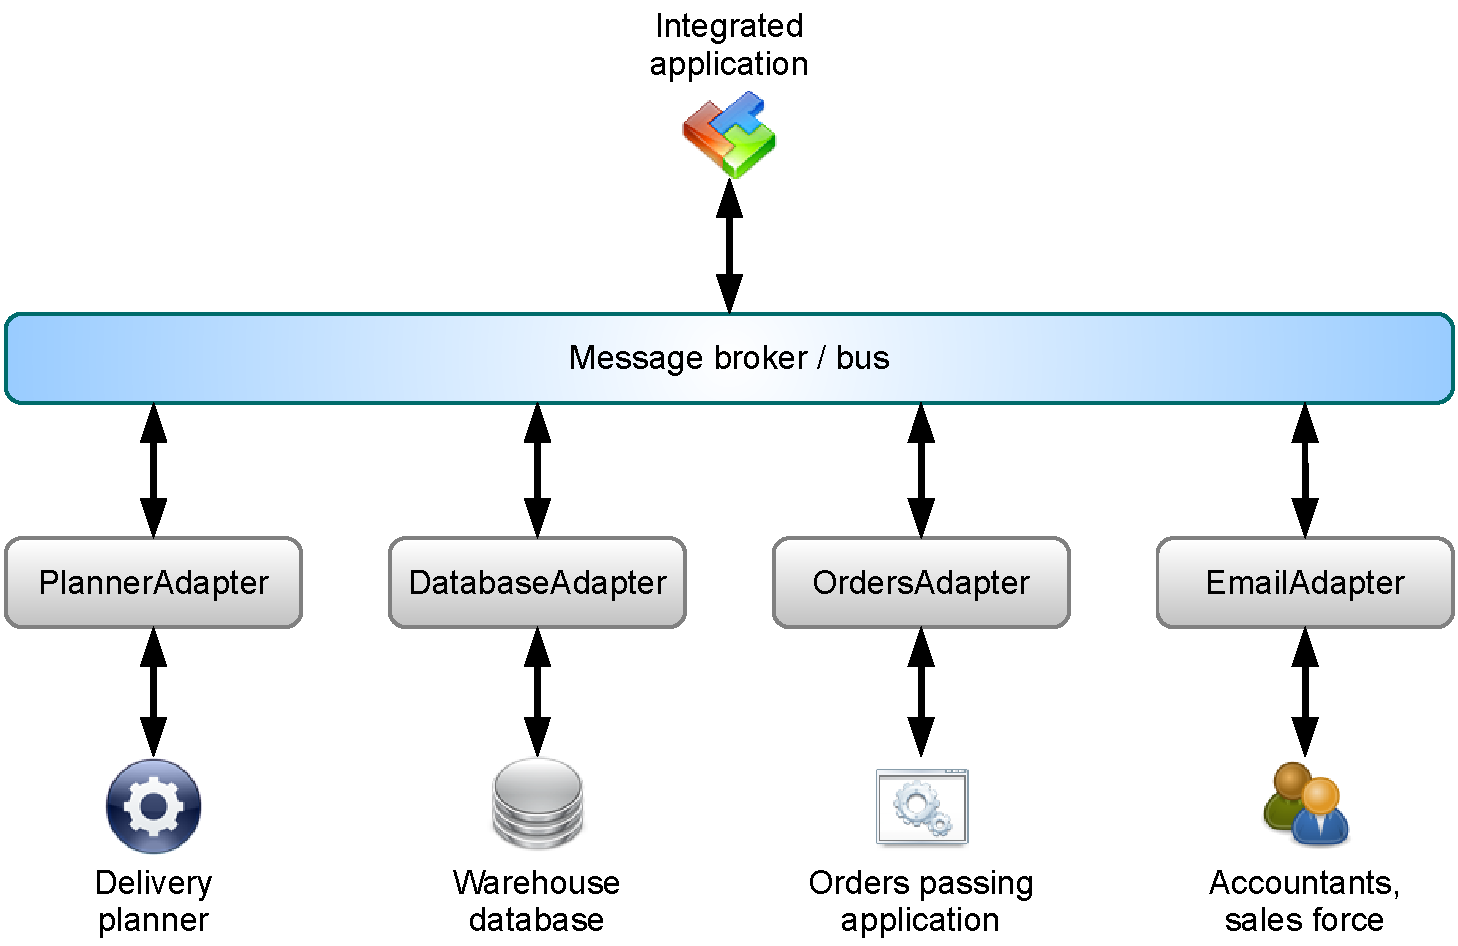
\includegraphics[width=\textwidth]{content/web-services/eai-scenario}
    \caption{Enterprise application integration using a message broker / bus.}
    \label{fig:eai-scenario}
\end{figure}

\paragraph{Example.}
We give an example of an enterprise application integration on Figure~\ref{fig:eai-scenario} where the business process of the purchase orders management is handled through a set of existing applications. Each application is connected through an adapter to a message-oriented middleware, called a \emph{messages bus}. Each message is routed (and possibly transformed) to other entities (e.g., a message sent by the orders passing application for asking goods availability is delivered to the warehouse database adapter). Each adapter is using diverse forms of middleware to bridge the bus and the application. For example the warehouse database adapter can use an ODBC connection to deal with the underlying database, while the delivery planner adapter may use RPC to communicate with the plannification system.

\paragraph{Limitations of conventional middlewares}
The ``conventional'' middlewares that we saw above all share some common limitations. The first one is probably that a lot of adaptation components have to be developed to allow two middleware-based systems to ``talk'' to each other. Another issue is that conventional middlewares are largely centralized \cite{Alonso04}, which limits deployment flexibility and again, requires the development of adapters. As an example, given two RPC frameworks, there is often a need for creating an adapter if they come from different vendors. Worse, even a standard specification is not enough for granting interoperability of systems. A good example is the Java Messaging System (JMS) that defines a standard API for MOM middleware in Java. While every JMS-compliant implementation ensures that an application can be ported from one JMS vendor to another one, there is no requirement on the network protocols and data representation formats, meaning that adapters have to be developed to bridge JMS brokers originating from different vendors.

Things get worse when integration needs to be performed across the boundaries of organizations, as network connectivity issues get added to the (already costly) development of adapters. Indeed, crossing companies firewalls is a serious concern as security need to be preserved, and maintaining such exceptions is complex. Also, a company will rarely trust a partner enough for allowing a direct connexion between their information systems: connectors also need to provide a controlled, coarse-grained interface to the internal information system. Another issue is that in such cases, integration is performed in a point-to-point fashion, something that does not scale well as the number of integrated partners grows \cite{Alonso04}. There is also an inherent lack of flexibility in those approaches as developing adapters and allowing basic connectivity takes time. By contrast, organizations today want to reduce costs, integrate easily with partners and be able to change and outsource some of their assets ``painlessly''.

Web services, and more generally service-oriented architectures have most benefits of the previous middleware families for facilitating application integration. But better, they also solve the mentioned limitations as we will see now.

% ........................................................................... %

\section{Service-oriented computing}

% ........................................................................... %

This section presents service-oriented computing. We start by an overview of service-oriented architectures. We then review the existing web service technologies before looking at service descriptions.

% ........................................................................... %

\subsection{Service-oriented architectures}

% ........................................................................... %

A commonly-accepted definition\footnote{\url{http://webservices.xml.com/pub/a/ws/2001/04/04/webservices/index.html} and \url{http://www6.software.ibm.com/developerworks/education/wsbasics/wsbasics-ltr.pdf}} of web services is the following:
\begin{quote}
\textsl{
Web services are a new breed of Web applications. They are self-contained, self-describing, modular applications that can be published, located, and invoked across the Web. Web services perform functions, which can be anything from simple requests to complicated business processes... Once a Web service is deployed, other applications (and other Web services) can discover and invoke the deployed service.
}
\end{quote}\

Service-oriented architectures (SOA) form the new wave of information systems \cite{PTDL07,PH07}. The key idea of SOA is to turn the data sources and applications in an enterprise system into  distributed units referred to as \emph{services}. Each service is self-described and it is expected to fulfill a very focused set of coarse-grained functionality requirements (e.g., a payroll processing service is not expected to also handle warehouse provisioning). They can then be assembled to realize applications and business processes. Services provide standard-based, platform-neutral interfaces that hide the implementation details. Also, the services should be autonomous with little dependencies to each other. This means that SOA promotes the loose coupling of services that are used for performing application integration of heterogeneous assets. The loose-coupling comes from both the fact that services are autonomous and that they use open standards for their external access (interfaces and data exchange formats).\\

While approaches with similar goals had been developed before the advent of web services (e.g., Corba, distributed components, ...), they bring some novelty \cite{Alonso04}. SOA are indeed often associated with web services as the core mean to realize them. Instead of re-inventing new interface specifications and data encoding means, they directly use widespread, ubiquitous standards such as XML or HTTP. The entry ticket to those technologies is rather low compared to previous approaches, which makes it possible to reuse legacy applications, hide their implementation (including the languages and platform choices) and integrate them with other applications also exposed as services. Another significant improvement in terms of application integration is that SOA blur the traditional boundaries of information systems. Indeed, integrating the information systems of different organizations has traditionally been a costly, largely ad-hoc process \cite{EAA02}, as information systems rarely rely on the same technological choices (e.g., languages, platforms) and normative choices (e.g., data representation formats, schema). Technologies such as web services naturally cross networks without having to develop network-specific bridges (e.g., virtual private networks) and as such, they make it ``natural'' to integrate the heterogeneous information systems of different organizations.\\

\begin{figure}[htbp]
    \centering
    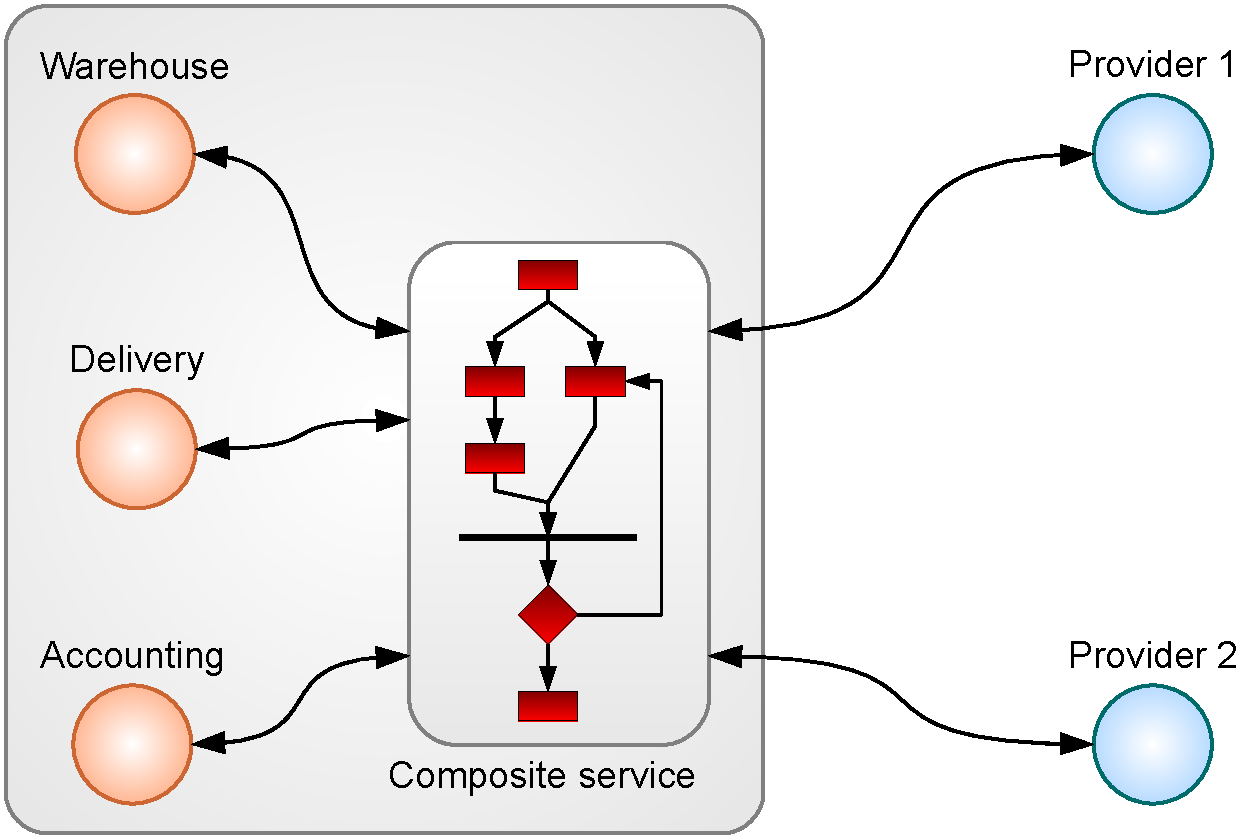
\includegraphics[width=\textwidth]{content/web-services/soa-composition-scenario}
    \caption{A SOA composition scenario.}
    \label{fig:soa-composition-scenario}
\end{figure}

We give an example of a simple service-oriented architecture on Figure~\ref{fig:soa-composition-scenario}. Three in-house services are provided: a warehouse management service, a delivery service and an accounting service. Each of them is an interface to larger applications and data sources and may well have been implemented using different technologies. There are also two external services of providers. A composite service is created by using an orchestration described by a BPEL process (which is not detailed on the figure). When a purchase order is received, it first checks with the warehouse for availability. If not, a quote is asked to each provider for provisioning the warehouse with the cheapest offer. Once this is done, goods are removed from the warehouse for delivery and the payment is delegated to the accounting.
%
In this example, it is possible to externalize the accounting of the organization very quickly: all that is needed is that the accounting provider offers a service with a compatible interface (or more realistically with minimal adaptation required). This is by itself a significant improvement over traditional integration across enterprise information systems.

% ........................................................................... %

\subsection{Technologies}

% ........................................................................... %

We now give an overview of the main web services technologies.

\paragraph{XML-RPC.}
XML-RPC is the first form of web services to have appeared. Defined in \cite{DW98}, it is a small and simple specification for performing RPC-style communications between systems. As the name suggests, the marshaling and unmarshaling of the invocations are done using XML for data representation. The marshaled messages are conveyed using the HTTP protocol (HTTPS can be used for secure point-to-point communications). Both the limited data types and the general minimalism in XML-RPC have facilitated its widespread adoption.

\paragraph{SOAP.}
SOAP \cite{MGMH+03} is a standard protocol defined by the W3C for exchanging XML-based messages between web services and their requesters. It builds on top of widespread existing standards such as XML, URI, HTTP and SMTP. Basically, a SOAP message is an XML document that acts as an envelope for the content being sent. In turn, a SOAP message is meant to be transported over various kind of protocols, the most used being HTTP / HTTPS. While the usual expected alternative is the \emph{Standard Mail Transfer Protocol} (SMTP), real-world applications have been using IIOP (from Corba), XMPP (Jabber open instant messaging) or even JMS (\emph{Java Messaging System}) to route SOAP messages. SOAP messages can be used either to simulate RCP-style communications, or document-style communications which are analogous to asynchronous messaging systems.

\begin{figure}[htbp]
    \centering
    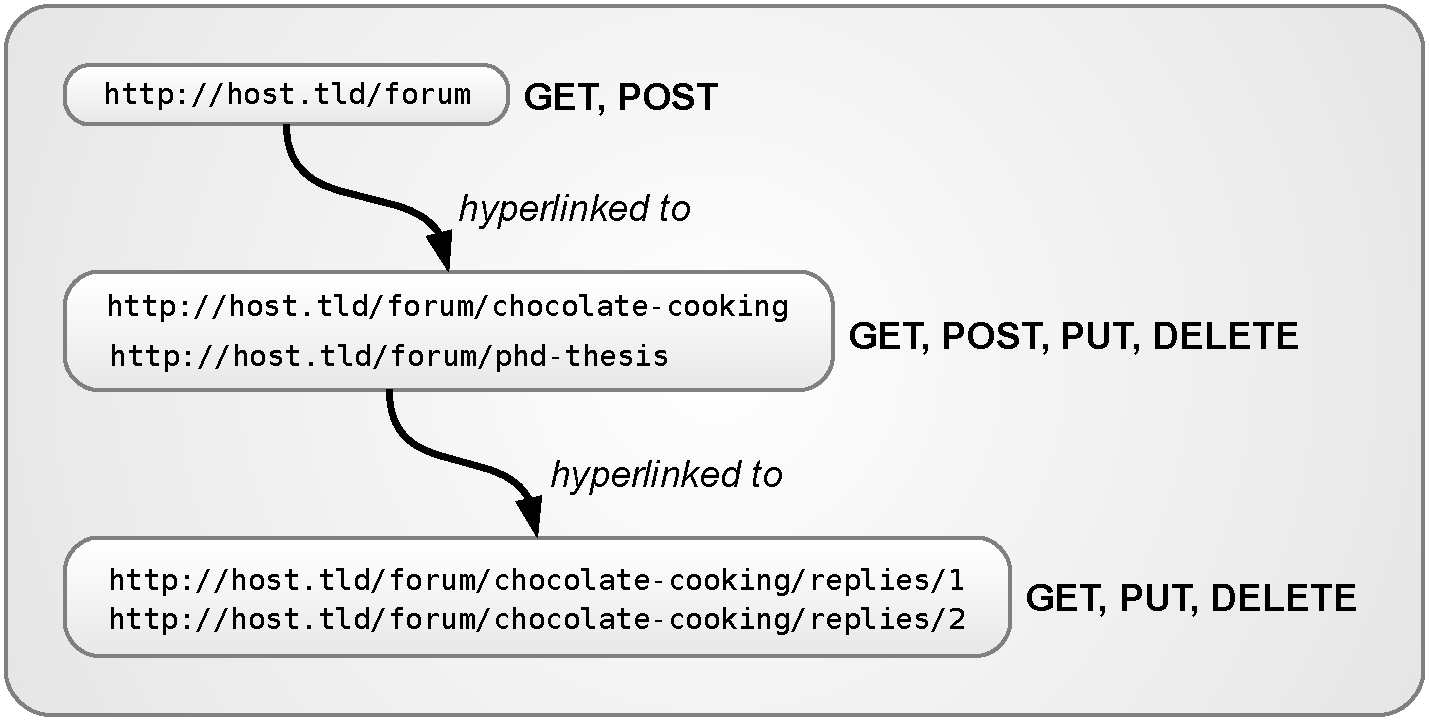
\includegraphics[width=\textwidth]{content/web-services/restful-forum}
    \caption{A \emph{RESTful} forum application.} 
    \label{fig:rest-forum}
\end{figure}

\paragraph{REST.}
The concept of REST\footnote{REST stands for \emph{\textbf{RE}presentational \textbf{S}tate of \textbf{T}ransfer}.}-style services first appeared in \cite{RTF00}. It is not a formal specification of a technology for building web services. Rather, it is an architectural style for building web services that emphasizes the semantics of both the HTTP protocol and the \emph{Universal Resource Identifiers} (URIs).
The core concept behind REST is that applications expose \emph{resources} that are accessible through URIs over the HTTP protocol. A resource may have several \emph{representations}, i.e., it may use different data encodings (e.g., XML, CSV, plain text) to accommodate different requesters. The resources can be \emph{hyperlinked} with each other and manipulated through a limited set of \emph{verbs}: the HTTP protocol methods (\textsf{GET}, \textsf{POST}, \textsf{PUT} and \textsf{DELETE}, see \url{http://www.w3.org/Protocols/rfc2616/}). As such, resources provide a \emph{uniform interface} to applications \cite{RTF00}.
We give an example of a \emph{RESTful}\footnote{Widely-used jargon for touting an application as being designed using the REST philosophy.} forum application on Figure~\ref{fig:rest-forum}. Hyperlinked resources can be manipulated by a HTTP software agent (e.g., for fetching message threads or posting a reply).

\begin{figure}[htbp]
    \centering
    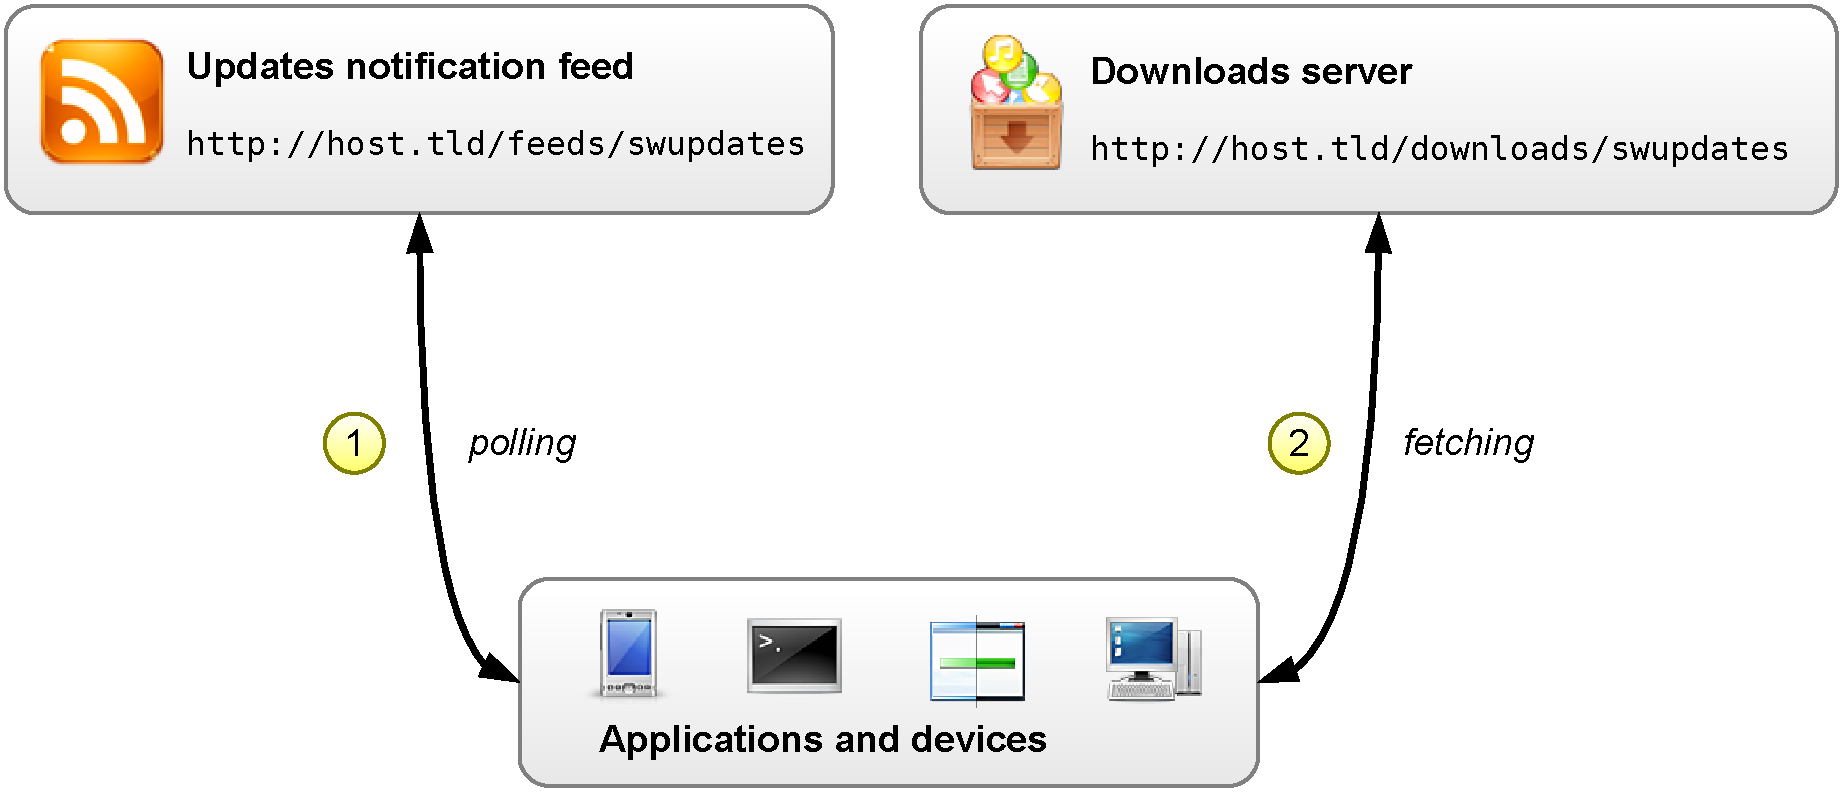
\includegraphics[width=\textwidth]{content/web-services/syndication-scenario}
    \caption{A simple software updates notification and distribution scenario based on syndication.} 
    \label{fig:syndication-scenario}
\end{figure}

\paragraph{Syndication feeds.}
Syndication web services have become increasingly popular with the rise of collaborative online applications such as blogs, wikis and podcasting. They provide resources called \emph{feeds} to notify \emph{subscribers} of events (e.g., a new blog post is available). The service does not directly notifies the subscribers of changes. Rather, it provides a URL-accessible resource which is updated when needed. Subscribers poll the resource for changes on a periodical basis. Two XML-based specifications are currently competing. An example is given on Figure~\ref{fig:syndication-scenario} where a feed is made available for publishing software update notifications.

% ........................................................................... %

\subsection{Service description and discovery}

% ........................................................................... %

We now briefly review standards and specifications for describing static web services interfaces and discovering them.

\paragraph{Static interface.}
The \emph{Web Services Description Language} (WSDL) \cite{ECFC+01} is an important add-on to SOAP-based web services. It provides a description of the static interface of such a service, much like IDL can be used in component technologies. As such, it specifies the operations supported by the service, the data schemas, and the binding information used to communicate with the service such as the transport protocol being used (ex: HTTP) and the location of the service (in the case of HTTP as a transport protocol, a URL). The messages that can be exchanged between a requester and a service are described using XML Schema (\url{http://www.w3.org/XML/Schema}).

A WSDL document can be used to bind to a SOAP-based service in two ways: either client invocation source code can be generated from the WSDL, or the binding can be performed dynamically at runtime. The latter case is especially possible with dynamic and reflexive languages such as \emph{Java} or \emph{Ruby}, by using the \emph{Proxy} design-pattern \cite{Gamma95}. Once either the static or dynamic binding has been performed, the service can be invoked.

\paragraph{Registries.}
The \emph{Universal Description, Discovery and Integration (UDDI) protocol} (see \url{http://www.uddi.org/}) provides a way for repositories to contain service functional and non-functional descriptions. Ultimately, a client interested in a given discovered service is able to obtain its WSDL description and bind to it after having found it. Another proposal for services repositories can be found in \emph{ebXML} (see \url{http://www.ebxml.org/}).

\paragraph{WS-*.}
Several specifications are gravitating around the SOAP web services stack \cite{HMBBFC+06}, often referred to as ``WS-*'' specifications. Most of them are actually irrelevant with no practical adoption in real-world use-cases \cite{WS-standards}. Among the very few relevant ones we have:
\begin{itemize}
  
  \item WS-Security (\url{http://docs.oasis-open.org/wss/v1.1/}), a specification for end-to-end preservation of the messages confidentiality and authenticity
  
  \item WS-Addressing (\url{http://www.w3.org/Submission/ws-addressing/}), which defines a standard representation for endpoint references and routing schemes (useful for correlation in stateful web services)
  
  \item WS-Policy (\url{http://www.w3.org/Submission/WS-Policy/}), a standard representation of quality of service requirements (e.g., security, message-encoding optimizations, ...)
  
  \item WS-Reliability (\url{http://docs.oasis-open.org/wsrm/ws-reliability/v1.1}) is useful for ensuring that messages are properly delivered in contexts that are not point-to-point communications between the service provider and its requesters
  
  \item WS-Coordination (\url{http://docs.oasis-open.org/ws-tx/wscoor/2006/06/}) and WS-Transaction (\url{http://dev2dev.bea.com/pub/a/2004/01/ws-transaction.html}) allow the coordination of web services.
  
\end{itemize}

The next section presents the model of business protocols \cite{FTBB} that serves as a foundation of this thesis work as it is suitable for describing the external behavior of a service with respect to the conversations it supports.

% ........................................................................... %

\section{Business protocols}

% ........................................................................... %

Static interface descriptions such as WSDL are essential for facilitating the use of web-service based technologies. There is however a strong need for abstractions of a higher-level than just ``data formats and message names''. As such, there is a consensus over the need for also specifying the dynamic interface of services \cite{PTDL07,PH07,ws_cacm_special_issue}. In particular, the externally-observable behavior of a service is important for avoiding invalid conversations between a service and its requesters. For example, a service may offer to add goods to a shopping cart and make a payment. A WSDL document of such a service would give the related message names (e.g., \emph{addGoods} and \emph{pay}) as well as their XML schema. This is clearly insufficient as for instance, paying before adding goods is most often not a valid business process.

This section first recalls the business protocol model and its usefulness. It then presents protocol-based analysis before providing a discussion.

% ........................................................................... %

\subsection{Model}

% ........................................................................... %

The model of business protocols of \cite{FTBB,BBFC04,BCT-CAISE03,KBBB+04} is the foundation of the work being presented in this thesis. This model captures all of the conversations that a service supports, i.e., the set of ordered message exchanges that are valid (e.g., a purchase order should not be exchanged before an authentication message). As such, it provides an abstraction for capturing a service external behavior, allowing potential requesters to know how to avoid generating invalid conversations, which is by itself a significant enhancement compared to having ``just'' a WSDL description. The model is based on state-charts as it is commonly accepted as a suitable model for describing behaviors, but alternatives could have been used as well such as Petri-nets or abstract BPEL (the later capture the operations orderings in a BPEL process).\\

\begin{figure}[htbp]
    \centering
    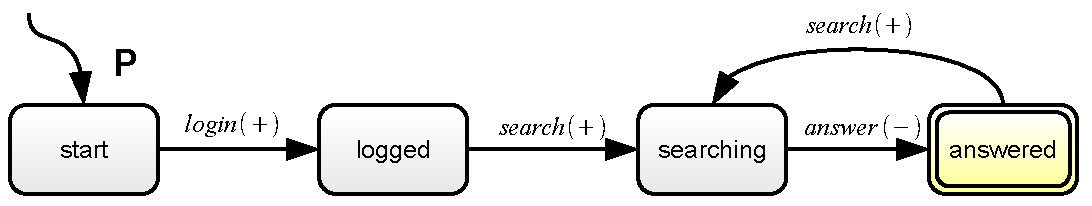
\includegraphics[width=\textwidth]{content/web-services/business-protocol}
    \caption{A business protocol of a search engine.} 
    \label{fig:business-protocol}
\end{figure}

As an example, Figure~\ref{fig:business-protocol} shows a business protocol of a search engine. States represent the various stages a service may go through while transitions are triggered when a message is received or sent. There is a unique initial state and many final states. In this protocol, conversations start with the service receiving a \texttt{login} message (the polarity $(+)$ is used to indicate that the message is incoming). Following that, a search can be performed and the results can be retrieved through repeatable sequences of \texttt{search} -- \texttt{answer} messages (again, the polarity $(-)$ is used for messages that are emitted by the service). The \textsf{answered} state is final: every conversation that ends in this state is said to be valid. By contrast, an invalid conversation would be $\mathtt{search} \cdot \mathtt{login} \cdot \mathtt{answer}$. Finally, it should be noted that state names do not have much importance in the model as conversations are about messages being exchanged.\\

Business protocols can be useful in several analysis contexts, both at development and runtime \cite{FTBB,BBFC04,BCT-CAISE03,KBBB+04}. Conformance checking is useful for a service provider to check if the actual implementation of a service meets a specification which can be either provided to clients (e.g., in the documentation), or imposed from standards (e.g., RosettaNet PIPs \cite{ROSETTANET}). Another one is for a requester to check that its own client protocol is compatible with a service, and if it is not, perform some adaptations so as to accommodate the service protocol to avoid errors. Finally, there are cases were a service needs to be replaced (e.g., failures, business-driven need for changing partners, etc). Replaceability analysis is useful so that a new service can be used as an alternative with minimal impacts on the existing requesters. Especially, it helps in identifying the potential mismatches at the protocol level so that adapters can be created. As such, both compatibility and replaceability analysis can be interesting as part of a service discovery process. In this work, we are interested in protocol-based compatibility and replaceability analysis that we outline hereafter.

% ........................................................................... %

\subsection{Protocol analysis}

% ........................................................................... %

Business protocols allow to perform fine-grained types of compatibility and replaceability analysis to see if (and how) two services can have interactions based on their protocols (compatibility), or if a service can be replaced transparently by another one for its current requesters (replaceability). Several classes of both compatibility and replaceability have been defined.
\begin{itemize}

	\item \emph{Partial compatibility} between two protocols $\mathcal{P}_1$ and $\mathcal{P}_2$ implies that at least one conversation can be carried out between two services implementing these protocols.

  \item A protocol $\mathcal{P}_1$ is \emph{fully compatible} with $\mathcal{P}_2$ if $\mathcal{P}_2$ can support all message exchanges that $\mathcal{P}_1$ can generate (the inverse is not necessarily true).
  
  \item \emph{Protocol equivalence} occurs when two protocols support exactly the same conversations.
	
	\item \emph{Protocol subsumption} occurs when a protocol supports at least all of the conversations of another one.
	
	\item \emph{Protocol replaceability w.r.t. a client protocol} occurs when a protocol $\mathcal{P}_1$ can replace a protocol $\mathcal{P}_2$ when interacting with a client protocol $\mathcal{P}_c$ if every valid conversation between $\mathcal{P}_2$ and $\mathcal{P}_c$ is also a valid conversation between $\mathcal{P}_1$ and $\mathcal{P}_c$.
	
	\item \emph{Protocol replaceability w.r.t. an interaction role} is similar to the previous one. It occurs when a protocol $\mathcal{P}_1$ can replace a protocol $\mathcal{P}_2$ if $\mathcal{P}_1$ behaves like $\mathcal{P}_2$ when $\mathcal{P}_2$ behaves as an interaction role $\mathcal{P}_r$.

\end{itemize}

Those analysis classes are characterized by using a set of protocol operators.
\begin{itemize}

	\item The \emph{intersection} operator computes the common conversations that two services support.
	
	\item The \emph{parallel composition} operator computes the common interactions that can take place between two services.
	
	\item The \emph{difference} operator computes which conversations are supported by a given service, but not by a second one.

\end{itemize}

\begin{figure}[htbp]
    \centering
    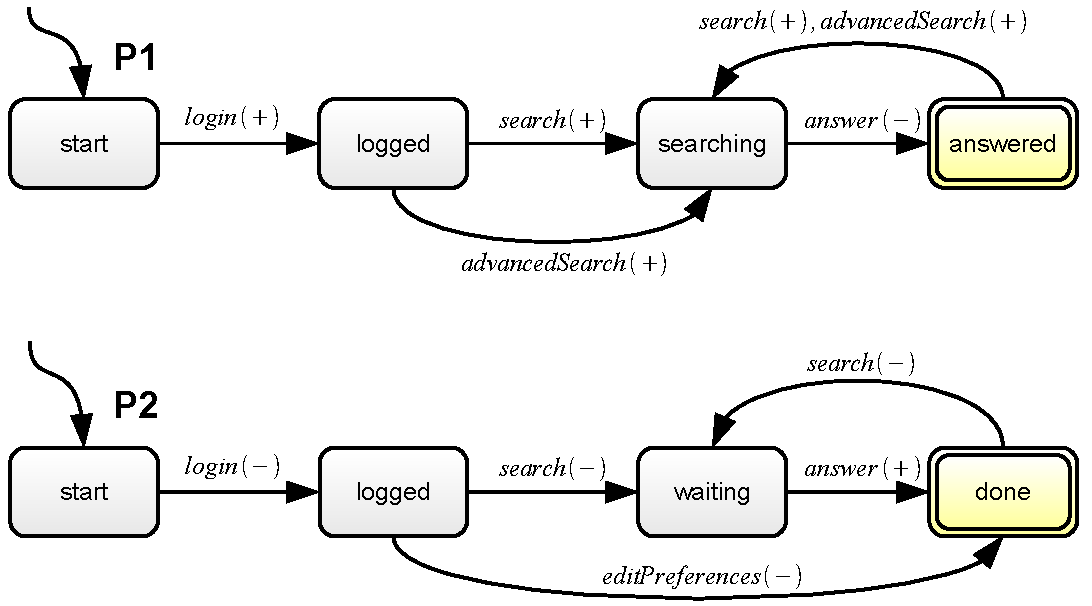
\includegraphics[width=\textwidth]{content/web-services/business-protocol-analysis}
    \caption{Two business protocol for illustrating analysis.} 
    \label{fig:business-protocol-analysis}
\end{figure}

As an example, two services are partially compatible as long as their parallel composition yields a non-empty protocol (i.e., at least one conversation is supported). This is the case between the protocol $P$ of Figure~\ref{fig:business-protocol} and $P_2$ of Figure~\ref{fig:business-protocol-analysis}. They are however not fully compatible as $P_2$ can generate some conversations that $P$ cannot support (e.g., $P$ does not support \texttt{editPreferences} messages).

In terms of protocol replaceability, the protocol $P$ of Figure~\ref{fig:business-protocol} can be replaced by the protocol $P_1$ of Figure~\ref{fig:business-protocol-analysis}. Indeed, there is protocol subsumption of $P$ by $P_1$. The two  protocols are however not equivalent as $P$ does not support \texttt{advancedSearch} messages: $P$ cannot replace $P_1$.

% ........................................................................... %

\subsection{Discussion and related work}

% ........................................................................... %

The following discussion first reviews common model families as business protocols opted for a state-based model. Notions such as orchestration, choreography and models for service abstractions are then briefly reviewed. Finally, research projects for web services life-cycle management are mentionned.

\paragraph{Model families.}
We consider the following three families: state-based models, activity-based models and rule-based models. 
State-based models can be found in a variety of contexts, mainly for describing behavioral abstractions of a system. In particular, the UML models family \cite{UML} contains several of them, acting as different ``facets'' over the representation of a system depending on the type of information that is to be captured (i.e., the general system behavior, the system behavior in a specific choreography, etc). We briefly recall the most important of them.
\begin{itemize}

    \item Collaboration diagrams
    allow to represent the message exchanges between several (distributed) entities. Arrows are drawn between the entities, carrying both a message and number. The number (part of a total order) is used to define the messages chronology of the collaboration that is being modeled.

    \item Sequence diagrams
    are similar to the collaboration diagrams except that they use \emph{lifelines} to denote when the object representing the entities are instantiated and discarded. Messages are exchanged between those lifelines, optionally having a number as in the case of collaboration diagrams. Indeed, the message exchange arrows are usually sorted vertically by chronological order.

    \item Statecharts
    capture all of the possible states of a given entity. The transitions between states are triggered on events (for example a message is received).

\end{itemize}

Activity-based models have been used to represent systems in an executable form (e.g, workflow management systems \cite{aalst98application}). States represent activities, and the transitions are triggered when the activities are finished. Each entity is given a \emph{swimlane}, and an activity belongs to the swimlane of the executing entity. In some of those models, the transitions can carry data flows.

Rule-based systems \cite{Forgy79,Forgy82} define behavior through a set of \emph{rules}. A rule is triggered when a given \emph{event} occurs, or when a given \emph{condition} is met. The rule then defines an action which is executed. Rule-based systems have been widely used where the systems behavior need frequent updates from domain experts writing the rules in domain-specific languages.

We chose to base our model upon the state-machine formalism. Indeed, it is commonly used to model the behavior of systems, due to the fact that it is simple and intuitive. Activity-based models are more suitable for creating executable models. Finally, rule-based models are a natural fit for complex decision-making systems where the logic must be frequently updated (e.g., by business analysts, accountants, etc.). They are however less suitable for describing behaviors.

\paragraph{Models for service abstractions.}
Research on web services has naturally lead to various models being proposed for capturing different types of abstractions. A discussion on modeling web services interactions has been proposed in \cite{TB-WWV06} and is further discussed in \cite{BSF06}. An approach for web services interfaces was defined in \cite{DBACTH05}. A model with similar goals as timed protocols had been introduced in \cite{berardi03finite}, but the timing constraints defined in the model have yet to be taken into account. A language for web services choreographies called \emph{Chor} has been proposed in \cite{QZCY-WWW07} as a simplification of WS-CDL.
WS-CDL (see \url{http://www.w3.org/TR/ws-cdl-10/}) is the reference specification for choreographies. Tools leveraging WS-CDL for facilitating development of SOA systems are currently emerging \cite{KangWH07}. BPEL also offers \emph{abstract process} for describing the externally observable behavior of a service composition. Lesser-known alternatives to BPEL include YAWL \cite{AalstADH04,AalstH05}, a general-purpose workflow language that has support for web services.

All of those approaches share many similarities with this work and the base model for business protocols of \cite{FTBB}. Surprisingly, little work has been done on timing abstractions. Also, those works do not provide a fine-grained range of compatibility and replaceability analysis classes, which makes our work original. Finally, business protocols and WS-CDL are complementary, not competing proposals.

\paragraph{Life-cycle management research projects.}
The \emph{ServiceMosaic project} \cite{BCTPM06-SM} aims at developing a model-driven framework for web service life-cycle management. It has a CASE tools set for supporting the service development life-cycle that includes facilities for modeling, analyzing, discovering and adapting web service models \cite{BCTPM06-SM,NezhadSBCPT07}. The work presented in this thesis is part of this project. ServiceMosaic is presented in larger details in chapter~\ref{chap:protocols-project}.

The \emph{Self-Serv} project was the precursor of the larger-scope ServiceMosaic project: \cite{ShengBDM02,BenatallahDM02,BenatallahSD03}. The goal of Self-Serv was to allow for rapid composition of web services through a declarative approach. The execution of the obtained composite services was made in peer-to-peer, dynamic environment.

The project called \emph{Astro} is another platform for the life-cycle management of web services \cite{TrainottiPCZLBBT05}. It features several contributions in the area of business requirements and verification, service synthesis and composition, and semantic web services. While it shares some similarities with ServiceMosaic (e.g., adaptation, supporting composition, Eclipse-based implementation), it focuses more on orchestration models (based on BPEL) than choreographies (e.g., the business protocol that a service supports). There is also no model discovery component such as the protocol discovery from execution log tools suite that ServiceMosaic provides \cite{Motahari-NezhadSBC07}. Finally, some works in Astro consider timing abstractions \cite{KazhamiakinPP06}. However, the work that is presented in this paper mainly reuses well-known timed automata model-checking techniques in service-based compositions. As we will see later, our approach makes a novel use of timed automata for obtaining the decidability and closure of protocol operators, not for performing straightforward, traditional model-checking. \\

While business protocols provide \emph{temporal constraints} (i.e., the messages ordering), they do not provide \emph{timing constraints} (e.g., a payment must be performed at most 48 hours after having purchased). This thesis revisits the concepts of business protocols modeling and analysis and enhances them using timing constraints. The result is a model that supersedes business protocols with added timing constraints and adapted analysis techniques. As we  established a link between our extended model and timed automata \cite{RADLD94} to obtain theoretical results on the time-aware analysis of protocols, we present them in the next chapter.

% ........................................................................... %
